\documentclass[aps,prd,twocolumn,superscriptaddress,preprintnumbers,floatfix,nofootinbib]{revtex4-2}

\usepackage{showyourwork}
\usepackage{amsfonts,amssymb,amsmath}
\usepackage[nolist,nohyperlinks]{acronym}

\newcommand*{\mi}[1]{\textsf{\color{magenta} [\textbf{MAX:} #1]}}

\begin{document}

\title{Constraining gravitational wave amplitude birefringence with GWTC-3}

\author{Thomas C. K. Ng}
\email{thomas.ng@link.cuhk.edu.hk}
\affiliation{Department of Physics, The Chinese University of Hong Kong, Shatin, Hong Kong}

\author{Maximiliano Isi}
\email{misi@flatironinstitute.org}
\affiliation{Center for Computational Astrophysics, Flatiron Institute, 162 5th Ave, New York, NY 10010, United States}

\author{Kaze W. K. Wong}
\email{kwong@flatironinstitute.org}
\affiliation{Center for Computational Astrophysics, Flatiron Institute, 162 5th Ave, New York, NY 10010, United States}

\author{Will M. Farr}
\email{wfarr@flatironinstitute.org}
\affiliation{Center for Computational Astrophysics, Flatiron Institute, 162 5th Ave, New York, NY 10010, United States}
\affiliation{Department of Physics and Astronomy, Stony Brook University, Stony Brook NY 11794, United States}

\date{\today}

\begin{abstract}
    The propagation of gravitational waves can reveal fundamental features of the structure of spacetime.
    For instance, differences in the propagation of gravitational-wave polarizations would be a smoking gun for parity violations in the gravitational sector, as expected from birefringent theories like Chern-Simons gravity.
    Here we look for evidence of amplitude birefringence in the latest LIGO-Virgo catalog (GWTC-3) through the use of birefringent templates inspired by dynamical Chern-Simons gravity.
    From 70 binary-black-hole signals, we obtain the most precise constraints on amplitude birefringence yet, an order of magnitude more stringent than previous results.
\end{abstract}

\maketitle

\begin{acronym}
\acro{GW}{gravitational wave}
\acro{GR}{general relativity}
\acro{CBC}{compact-binary coalescence}
\acro{BH}{black hole}
\acro{BBH}{binary black hole}
\acro{LVK}{LIGO-Virgo-KAGRA Collaboration}
\acro{PE}{parameter estimation}
\acro{FAR}{false-alarm rate}
\acro{GWOSC}{the Gravitational Wave Open Science Center}
\end{acronym}

\section{Introduction}
\label{sec:Introduction}
% Motivation
\Ac{GW} detections by the \ac{LVK} \citep{LIGO, Virgo, KAGRA} are now routinely used to test various aspects of Einstein's theory of \ac{GR} \citep{LIGOScientific:2016lio,LIGOScientific:2018dkp,LIGOScientific:2021sio}.
Among those, measurements of the basic properties of \acp{GW}, like their speed and polarization, can directly probe the fundamental symmetries of the underlying theory of gravity \citep{Will:2018bme}.
For instance, unequal propagation of \ac{GW} polarization states would reveal that spacetime is birefringent, a smoking gun for parity-odd theories like Chern-Simons gravity \citep{Jackiw:2003pm,Alexander:2009tp,Sopuerta:2009iy}.
Here we constrain the magnitude of possible amplitude birefringence using \ac{BBH} signals from the latest \ac{LVK} catalog, GWTC-3.

% Previous studies
Previous studies have constrained amplitude birefringence by performing different statistical analyses.
\citet{Yamada_2020} and \citet{Wang_2021} both performed \ac{PE} on the events in the first \ac{GW} transient catalog \citep{GWTC-1}, GWTC-1, using birefringent templates.
\citet{Okounkova_2022} considered the distribution of observed inclinations of the \ac{GW} events in the second \ac{GW} transient catalog \citep{GWTC-2}, GWTC-2, to look for signs of birefringence.

% What's new?
In this study, we used a frequency-dependent birefringence model to constrain the strength of \ac{GW} amplitude birefringence by performing \ac{PE}.
This model is a better approximation of the birefringence effect than the frequency-independent model used in \citet{Okounkova_2022}.
Compared to previous studies, we also performed \ac{PE} on more events, including events in the third \ac{GW} transient catalog \citep{GWTC-3}, GWTC-3.
We consider 70 binary black hole merger events with a \ac{FAR} $\leq1\mathrm{yr^{-1}}$.
These events are also listed in Table I in \citet{GWTC-3_population}.\footnote{
GW190720 is included in the list in \citet{GWTC-3_population}, but we did not include it in this study.
Details in Sec.~\ref{sec:GW190720}.}
We then give the population constraint on the strength of \ac{GW} amplitude birefringence by using the \ac{PE} results.

% Section guide
In Sec.~\ref{sec:Background}, we briefly review the background of \ac{GW} amplitude birefringence.
In Sec.~\ref{sec:Method}, we describe the modification we made to the waveform model, mention the configuration we used in the \ac{PE} and show the method we used to obtain the population constraint on \ac{GW} amplitude birefringence.
In Sec.~\ref{sec:Results}, we present the population constraint on \ac{GW} amplitude birefringence we obtained and show the results of individual \ac{PE}.
In Sec.~\ref{sec:Discussion}, we discuss the limitation of this study and provide suggestions for future studies.

\section{Background}
\label{sec:Background}

\subsection{Birefringence}
\label{sec:waveform}

% GW polarization
In \ac{GR}, \acp{GW} are comprised of two independent polarization modes, usually represented in the linear basis of plus ($+$) and cross ($\times$) states.
In the Fourier domain, they can be combined into left-handed (L) and right-handed (R) circular states \cite{Isi:2022mbx},
\begin{equation}
    h_{L/R} = \frac{1}{\sqrt{2}}\left(h_+ \pm i h_\times\right)\,,
\end{equation}
where $h$ is the frequency domain strain, with the plus and minus signs for L and R respectively.
These circular modes represent eigenstates of the helicity operator (helicity $\pm2$) and possess a definite parity.
Einstein's theory, which is parity even, predicts no difference in the dynamics of these two states.

% Waveform modification
Yet, parity odd extensions of \ac{GR} may make distinctions between the two circular polarizations, which can manifest in both the generation and propagation of \acp{GW}.
The latter can manifest in changes to the relative amplitude and phase of the polarizations that accrue as the wave propagates, giving us hope to detect initially small effects that compound over long propagation distances.

In particular, \emph{amplitude} birefringence would enhance one polarization mode over the other.
To first order in theories like Chern-Simons gravity, the Fourier-domain waveform observed a comoving distance $d_C$ away from the source takes the form of
\begin{equation}
    h_{L/R}^{\mathrm{br}}(f) =
    h_{L/R}^{\mathrm{GR}}(f) \times
    \exp\left(\pm\kappa\frac{d_C}{1\, \mathrm{Gpc}}\frac{f}{100\,\mathrm{Hz}}\right)\,,
    \label{eq:waveform_modification}
\end{equation}
where the emitted waveform $h_{L/R}^{\mathrm{GR}}$ is modified by an exponential birefringent factor to yield the observed waveform $h_{L/R}^{\mathrm{br}}$.
The overall magnitude of this effect for a given distance and frequency $f$ is set by a dimensionless opacity parameter, $\kappa$, which encodes the intrinsic strength of the birefringence.
The emitted waveform for a given source (i.e., the waveform observed very close to the source) will generally differ from the analogous waveform predicted by \ac{GR}; however, since we expect most viable modifications to \ac{GR} to be intrinsically small, it is standard to approximate the emitted waveform by the prediction from \ac{GR} (hence the notation ``$h^{\rm GR}$'' above).

Although the intrinsic modification is small, the effect targeted by Eq.~\eqref{eq:waveform_modification} accumulates as the \ac{GW} propagates.
During propagation, the effect of birefringence will be built up with the number of cycles which depends on the distance traveled and the frequency of the \acp{GW}.
According to Eq.~\eqref{eq:waveform_modification}, a positive $\kappa$ means the left-handed polarization is enhanced over the right-handed polarization, while a negative $\kappa$ means the opposite;
when $\kappa=0$, the observed waveform is the same as \ac{GR} predicts, meaning there is no birefringence.

Equation \eqref{eq:waveform_modification} can be derived as the first order effect in an expansion for multiple extensions of \ac{GR}.
In general, $\kappa$ will be a function of the theory parameters and the cosmological history, e.g., the value of the pseudo-scalar field and its derivative in Chern-Simons gravity.
Since it originates from an expansion, Eq.~\eqref{eq:waveform_modification} is a good approximation only for small exponents, 
\begin{equation}
\left|\kappa\right| \left(d_C/1\,\mathrm{Gpc}\right) \left(f/100\, \mathrm{Hz}\right) < 1\, .
\end{equation}
Otherwise, more frequency-dependent terms would enter the exponent of Eq.~\eqref{eq:waveform_modification} in a theory-dependent way.
\mi{specify what the parameter for the expansion is, add citations, and check with a theorist}

\subsection{Relation to inclination}

% Effect on inclination PE results
Under certain conditions, the effect of birefringence can be degenerate with a change in the orientation of the source with respect to the line of sight.
Concretely, for a nonprecessing compact binary inspiral in \ac{GR}, the observed amplitude ratio of the left-handed and right-handed polarizations is only a function of the inclination $\iota$, the angle between the orbital angular momentum of the source and the line of sight.
For  the dominant $\ell = |m| = 2$ angular mode of the radiation, the relation between the amplitude ratio and the inclination is
\begin{equation}
    \frac{h_{L}^\mathrm{GR}}{h^\mathrm{GR}_{R}}=\left(\frac{1-\cos\iota}{1+\cos\iota}\right)^2\,
\end{equation}
for all frequencies (see, e.g., Sec.~IIIC in \cite{Isi:2022mbx}).

Since birefringence impacts the observed amplitude ratio of left- and right-handed modes, it could also affect inferences about the source inclination \cite{Alexander:2009tp}.
However, the two effects are degenerate only if the frequency dependence of Eq.~\eqref{eq:waveform_modification} is neglected.
This is easy to see from Eq.~\eqref{eq:waveform_modification}, since the implied polarization ratio for the $\ell = |m| = 2$ mode of a nonprecessing source is
\begin{equation}
    \frac{h_{L}^\mathrm{br}}{h_{R}^\mathrm{br}}=\left(\frac{1-\cos\iota}{1+\cos\iota}\right)^2
    \exp\left({2\kappa\frac{d_C}{1\, \mathrm{Gpc}}\frac{f}{100\, \mathrm{Hz}}}\right)\, .
    \label{eq:modified_amplitude_ratio}
\end{equation}
For an isolated Fourier mode of definite frequency $f$, the effect of birefringence will be degenerate with a change in inclination; however, if multiple modes come into play, then no change in inclination can mask the effect of birefringence, which will generate dephasing in the time domain waveform (Fig~\ref{fig:birefringence_frequency_domain}).

\begin{figure}
    \script{birefringence_frequency_domain.py}
    \includegraphics[width=\columnwidth]{figures/birefringence_frequency_domain.pdf}
    \caption{
        The observed Fourier amplitude of two polarizations of a simulated GW signal with and without birefringence.
        The amplitudes, as GR predicts, are shown in dotted lines with blue and orange colors representing the left-handed and right-handed polarizations.
        The amplitudes with birefringence are shown in solid lines with blue and orange colors representing the left-handed and right-handed polarizations.
        This plot shows the effect of amplitude birefringence with frequency dependence.
        \mi{@Thomas can you add a panel with the time-domain waveforms (maybe just for L or R)?}
    }
    \label{fig:birefringence_frequency_domain}
\end{figure}

\citet{Okounkova_2022} took the effect of birefringence to be independent of the frequency, which is a zeroth-order approximation of the birefringence model in Chern-Simons gravity.
This assumption results in a full degeneracy between $\kappa$ and $\iota$:
to reconstruct the amplitude ratio from the interferometer data, an $\iota$ representing a more face-off inspiral can pair with a positive $\kappa$, or an $\iota$ representing a more face-on inspiral with a negative $\kappa$.
That fact can be used to constrain frequency-independent birefringence by searching for features in the distribution of inferred inclinations \cite{Okounkova_2022}.

By implementing Eq.~\eqref{eq:waveform_modification}, which is a first-order approximation of the birefringence model, we generally break the degeneracy between birefringence and source orientation; this was also the case in the frequency-dependent relations studied in \cite{Yamada_2020,Wang_2021}.
Nevertheless, there exist systems for which the degeneracy cannot be perfectly broken because not enough frequencies are available in the data.
As we will see in Sec.~\ref{sec:Results}, this is the case for heavy \acp{BBH}, which are only in the sensitive band of the detectors for a few cycles.


\section{Method}
\label{sec:Method}

\subsection{Single-event parameter estimation}

To constrain birefringence, we reanalyze events from GWTC-3 \citep{GWTC-2.1, GWTC-3} implementing Eq.~\eqref{eq:waveform_modification} to directly obtain a posterior on $\kappa$ from the strain of each event.
We analyze the 70 \acp{BBH} that were detected with $\mathrm{FAR} < 1/\mathrm{yr}$; to avoid extended computations on longer signals and considering these are generally at closer distances, we do not analyze systems involving neutron stars in this work.
We procure strain data from \ac{GWOSC} \citep{GWOSC}.

We carry out \ac{PE} using a custom version of \textsc{Bilby} \citep{Bilby}, that applies Eq.~\eqref{eq:waveform_modification} for any \ac{GR} baseline waveform.
We depart from the \ac{PE} configuration as in \citet{GWTC-2.1, GWTC-3, GWTC-2.1_dataset, GWTC-3_dataset}, with \textsc{IMRPhenomXPHM} as the reference waveform.
We apply a distance prior which is uniform in comoving volume and source frame time instead of a power law distribution used in \citet{GWTC-2.1, GWTC-3, GWTC-2.1_dataset, GWTC-3_dataset}, and set the prior on $\kappa$ to a uniform distribution between $-1$ and $1$.

For GW190521, we increase the maximum distance of the distance prior to $1.5$ times the original value, as the birefringence effect enables the probability of a larger distance.

In order to validate our \ac{PE} implementation, we reproduce the \ac{LVK} \ac{PE} results obtained assuming \ac{GR} by enforcing $\kappa = 0$; this also has the advantage of producing \ac{GR} runs that are directly comparable to our birefringent runs.
All our \ac{PE} results, including the \ac{GR} validation runs, are published in \citet{dataset}.

\subsection{Collective analysis}

\subsubsection{Shared birefringence parameter}

Since birefringence is a property of spacetime and we are targeting a propagation effect not intrinsic to any source, we should expect $\kappa$ to take the same value for all signals, whether it vanishes or not.
\mi{caveats?}
Under this assumption, the posterior on $\kappa$ inferred collectively from all events with a uniform prior is simply obtained from the product of the individual likelihoods, $p(d_i \mid \kappa) \propto p(\kappa \mid d_i)/p(\kappa)$, such that
\begin{equation}
    p(\kappa \mid \{d_i\})\propto p(\kappa) \prod_{i}\frac{p(\kappa \mid d_i)}{p(\kappa)}\,,
    \label{eq:restricted_posterior}
\end{equation}
where $d_i$ is the strain data for the $i$\textsuperscript{th} event, and $p(\kappa)$ is the prior on $\kappa$; since the prior is uniform, in our case Eq.~\eqref{eq:restricted_posterior} reduces to the product of the posteriors, namely $p(\kappa \mid \{d_i\}) \propto \prod_{i}p(\kappa \mid d_i)$.
We use Eq.~\eqref{eq:restricted_posterior} to obtain the primary constraint presented in this work.

\subsubsection{Nonshared birefringence parameters}

% Bayesian Hierarchical Modeling
In order to further characterize our set of measurements, and identify potential outliers, we carry out an additional collective analysis that allows $\kappa$ to take different values for each event \cite{Zimmerman:2019wzo,Isi:2022cii}.
To do this, we apply hierarchical Bayesian inference \cite{Loredo:2004nn} to model the distribution of $\kappa$'s consistent with the observed data:
we posit that there is a specific value of the parameter, $\kappa_i$, associated to each event, drawn from some unknown distribution of underlying values; from the imperfect measurements of $\kappa_i$ for each event, we may reconstruct the underlying distribution.
If we are interested in constraining the first two moments of the distribution, it is convenient to parametrize the $\kappa_i$'s as drawn from a Gaussian with unknown mean $\mu$ and variance $\sigma^2$, i.e., $\kappa_i \sim \mathcal{N}(\mu, \sigma^2)$ \cite{Isi:2019asy}, and measure those hyperparameters from the collection of observed data.

If \ac{GR} is correct and there is no birefringence, we should find the observed $\kappa$ distribution to be consistent with a delta function at the origin ($\kappa_i = 0$ for all $i$, or $\mu=\sigma=0$); on the other hand, if spacetime is birefringent, we expect to find a delta function at some nonzero value ($\kappa_i = \kappa \neq 0$, or $\mu = \kappa$ and $\sigma=0$).
But this analysis also has the power to reveal unexpected physics or systematics in our measurements: if $\sigma$ is confidently found to be nonzero, this would imply that our set of measurements are statistically unlikely to originate from a unique $\kappa$ value.
This could signal further physics than is implied by Eq.~\eqref{eq:waveform_modification} \mi{which physics? @Will, any ideas?} or, more prosaically, that there are outliers in our measurements due to mismodeling, e.g., in the waveform approximant or the noise of the detector.

Starting from the posterior on $\kappa$ from each event, the posterior on the hyperparameters $\mu$ and $\sigma$ can be calculated by
\begin{equation}
    p(\mu,\sigma \mid \{d\})\propto p(\mu,\sigma)\prod_{i}\int\frac{p(\kappa_i\mid d_i)}{p(\kappa_i)}p(\kappa_i\mid\mu,\sigma)\,d\kappa_i\,,
    \label{eq:posterior_of_mu_sigma}
\end{equation}
where $p(\kappa)$ is the prior initially applied to $\kappa$ during \ac{PE}, which in our case is a uniform distribution $\mathcal{U}[-1,1]$.
Furhter choosing the hyperpriors on $\mu$ and $\sigma$ to be uniform, Eq.~\eqref{eq:posterior_of_mu_sigma} simplifies to
\begin{equation}
    p(\mu,\sigma\mid\{d\})\propto\prod_{i}\int p(\kappa_i\mid d_i)\mathcal{N}(\mu,\sigma)\,d\kappa_i\,.
\end{equation}

We also calculate the expected population distribution of $\kappa$ marginalized over $\mu$ and $\sigma$.
This is given by
\begin{equation}
            p(\kappa\mid \{d\})=\int \mathcal{N}(\mu,\sigma)p(\mu,\sigma\mid \{d\})\,d\mu\,d\sigma\, , 
    \label{eq:generic_posterior}
\end{equation}
and represents our overall expectation for $\kappa$, given the observed set of individual measurements.
To sample the posterior distribution of $\mu$ and $\sigma$, we use the sampling package \textsc{flowMC} \citep{flowMC}.

\section{Results}
\label{sec:Results}
In this section, we present the results of our study.
We first show the PE results of all events and present the results of Bayesian hierarchical modeling.
Then, we will discuss some special events individually.

\begin{figure*}
    \script{violin_kappa.py}
    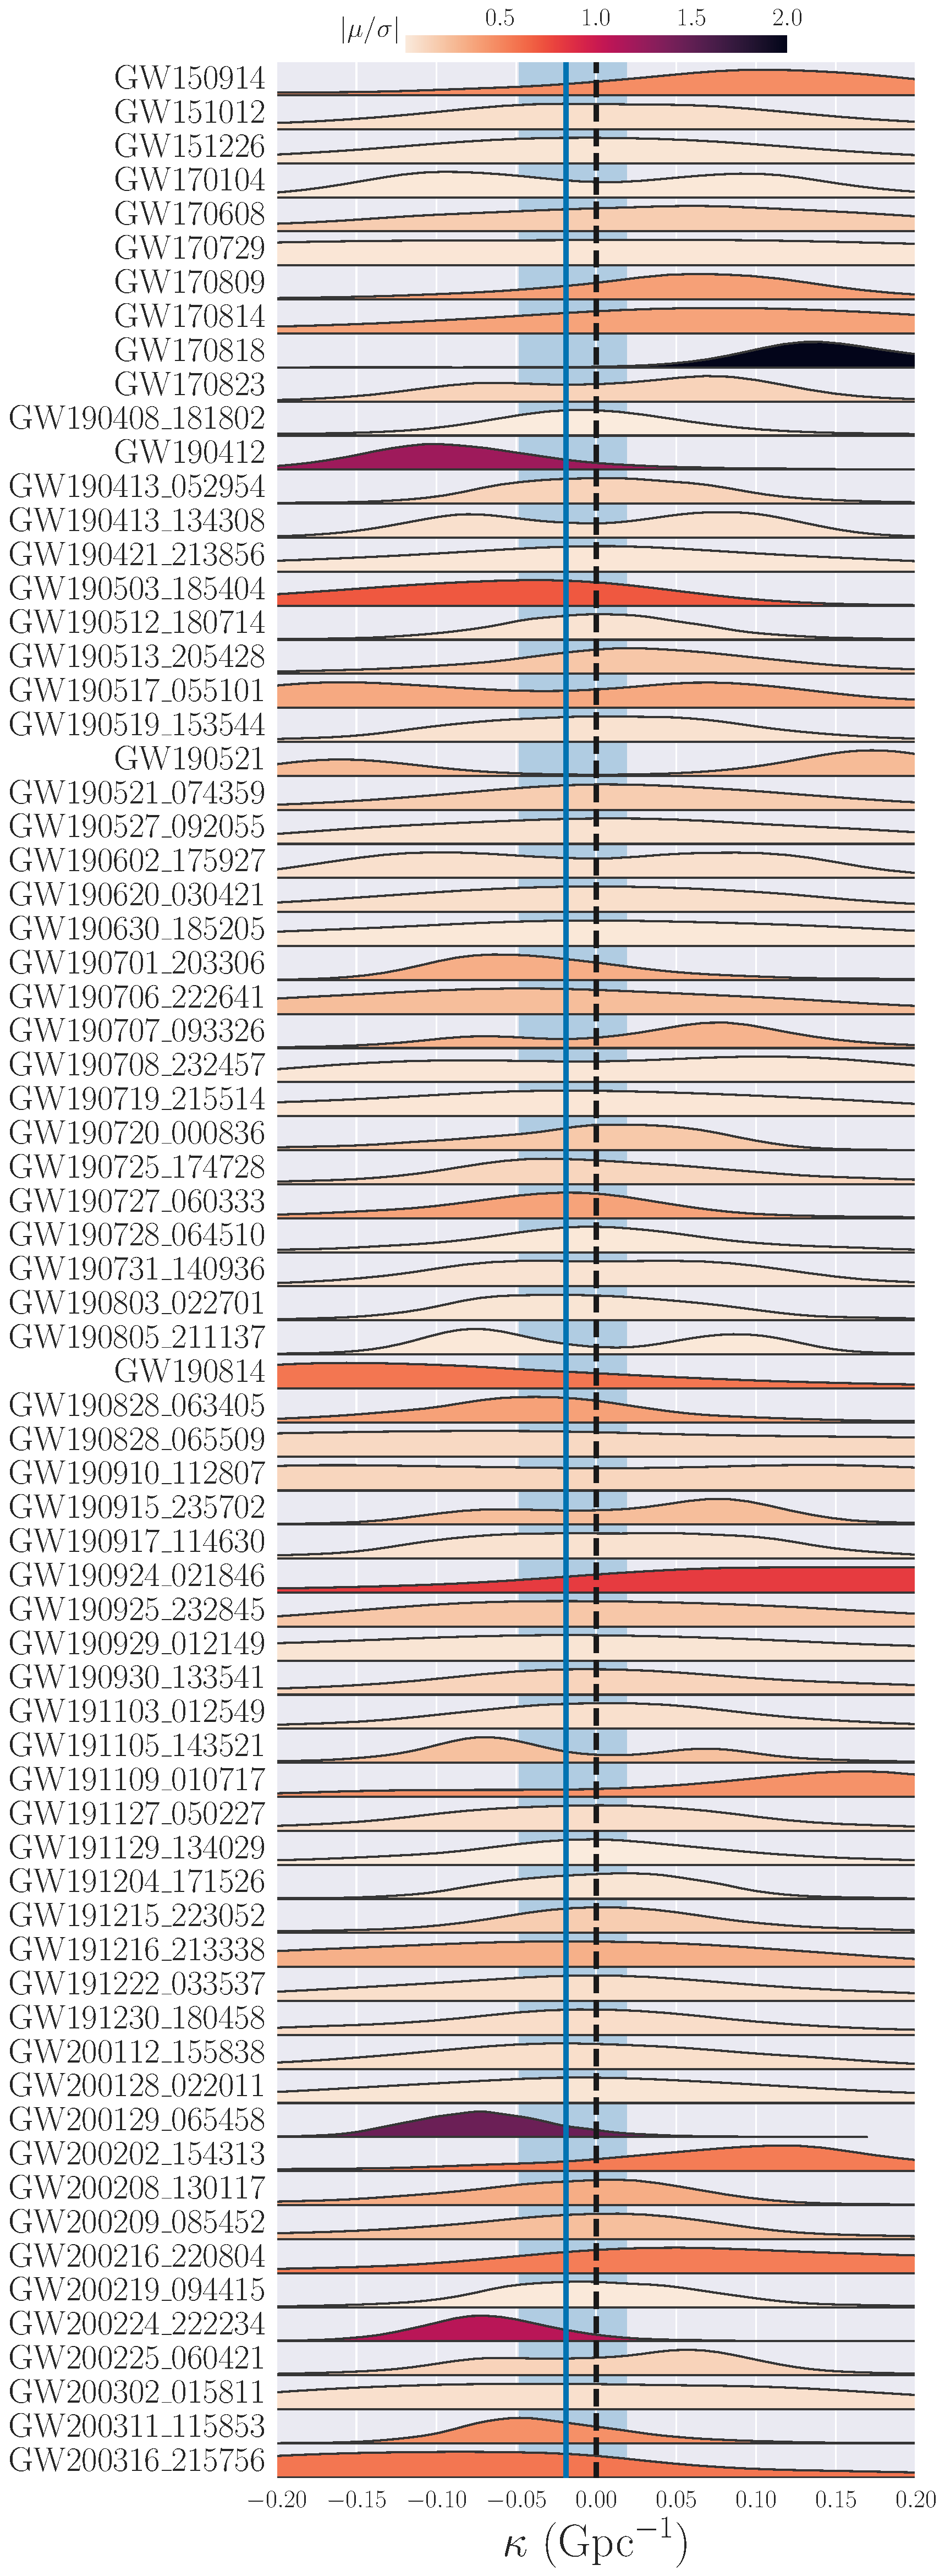
\includegraphics[width=\textwidth]{figures/violin_kappa.pdf}
    \caption{
        The violin plot shows the posterior of $\kappa$ for 70 events in this study.
        Each violin represents a different event.
        The color of the violins represents the quotient of the median and standard deviation of the posterior.
        The blue horizontal solid line represents the median of the restricted posterior of $\kappa$, and the blue dashed lines enclose the $90\%$ confidence interval of the restricted posterior of $\kappa$.
        The pink horizontal solid line represents $\kappa=0$.
        GW200129 is shown with light blue edges, as it is excluded from the calculation of collective analysis.
    }
    \label{fig:violin_kappa}
\end{figure*}

\subsection{Result on GWTC-3}
% Violin plot
In figure \ref{fig:violin_kappa}, we show the posterior of $\kappa$ for each event in the form of a violin plot.
The median and confidence interval of $\kappa$ are calculated with the restricted posterior distribution of $\kappa$, which is given by equation \ref{eq:restricted_posterior}.
We excluded GW200129 from the calculation of collective analysis.
Details of the exclusion are discussed in Sec.~\ref{sec:GW200129}.

\subsection{Bayesian hierarchical modeling}
% Corner plot of the mean and standard deviation of kappa
We then show the result of Bayesian hierarchical modeling in figure \ref{fig:corner_Gaussian}.
The median of $\mu$ within $90\%$ confidence interval is \variable{output/mu_median.txt}.
The median of $\sigma$ within $90\%$ confidence interval is \variable{output/sigma_median.txt}.
The posterior of $\mu$ is concentrated around $0$, which means the population constraint on $\kappa$ is consistent with GR.

\begin{figure}
    \script{corner_Gaussian.py}
    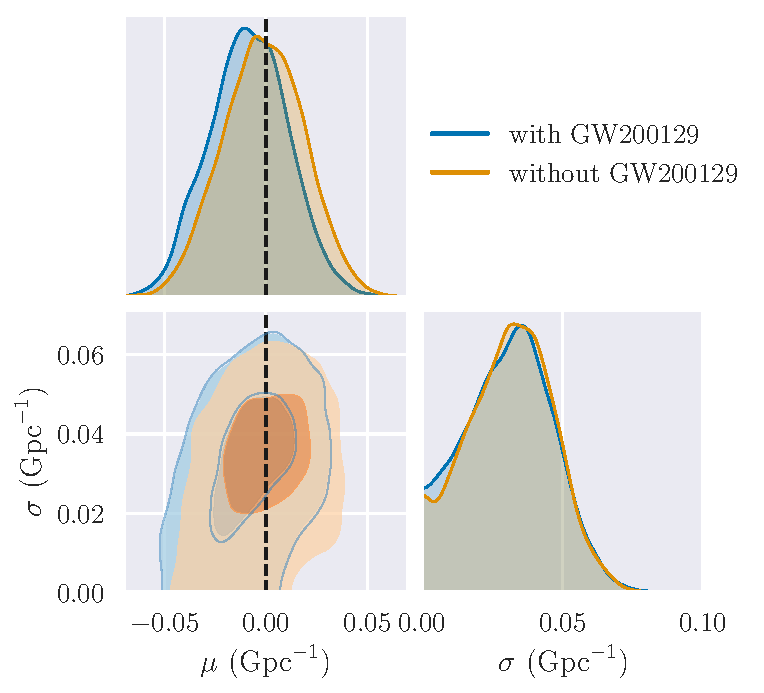
\includegraphics[width=\columnwidth]{figures/corner_Gaussian.pdf}
    \caption{
        The posterior of $\mu$ and $\sigma$ of the population distribution of $\kappa$.
        2D contour plot shows $39.35\%$ and $90\%$ confidence level.
        The orange line represents the median of $\mu$ and $\sigma$.
        The plot shows that the population constraint on $\kappa$ is consistent with GR.
    }
    \label{fig:corner_Gaussian}
\end{figure}

\subsection{Constaint on $\kappa$}
% Constraint on $\kappa$
In figure \ref{fig:posterior_kappa}, we show both the restricted posterior of $\kappa$ and the generic posterior of $\kappa$.
The restricted posterior is calculated by equation \ref{eq:restricted_posterior} with the assumption that $\kappa$ is a single value constant.
The generic posterior is calculated by equation \ref{eq:generic_posterior} with the assumption that $\kappa$ is a true value drawn from a Gaussian distribution.
The median of the restricted posterior within $90\%$ confidence interval is \variable{output/restricted_kappa_median.txt}.
The median of the generic posterior within $90\%$ confidence interval is \variable{output/generic_kappa_median.txt}.
Note that the result is consistent with GR when $\kappa=0$.
% talk about what events pull sigma in figure 2

\begin{figure}
    \script{posterior_kappa.py}
    \includegraphics[width=\columnwidth]{figures/posterior_kappa.pdf}
    \caption{
        The generic and restricted posterior of $\kappa$.
        The blue solid line shows the restricted posterior of $\kappa$, and the blue dashed lines enclose the $90\%$ confidence interval.
        The orange solid line shows the generic posterior of $\kappa$, and the orange dashed lines enclose the $90\%$ confidence interval.
        The pink vertical solid line represents $\kappa=0$.
    }
    \label{fig:posterior_kappa}
\end{figure}

% Case study

% Create sessions for all the outliers

% Case: GW170818
\subsection{Result on GW170818}

% Case: GW190412
\subsection{Result on GW190412}

% Case: GW200224
\subsection{Result on GW200224}

% Case: GW150914 (example of broken degeneracy)
\subsection{Result on GW150914}
In this study, we included frequency dependence of birefringence, which would affect the posterior of $\kappa$ obtained from PE.
Consider GW150914, the first GW detected by LIGO, as an example.
In figure \ref{fig:corner_GW150914}, we show the posteriors of the parameters of GW150914.
With the frequency-independent birefringence model, the posteriors for $\cos\iota$ look different from the posteriors assuming GR.
This is because, for a nonprecessing system, there is a degeneracy between $\kappa$ and $\iota$ if the frequency dependence is not included.
% explain the kappa gap

On the other hand, with the frequency-dependent birefringence model, the posterior looks similar to the GR posterior.
This is because the frequency dependence broke the degeneracy, as the effect of birefringence will differ from the effect of changing $\iota$.
In this case, the most probable value of $\kappa$ is close to $0$, which means the birefringence is weak or absent.
Therefore, the PE result with frequency dependence is consistent with GR.

\begin{figure}
    \script{corner_GW150914.py}
    \includegraphics[width=\columnwidth]{figures/corner_GW150914.pdf}
    \caption{
        The posterior of $\kappa$, luminosity distance $d_L$ and $\cos{\iota}$ for GW150914.
        Colors in the plot represent the PE result with GR done by LVK without cosmological reweighing \citep{GWTC-2.1, GWTC-3}, the PE results done by us with both frequency independent and dependent birefringence respectively.
        2D contour plot shows $39.35\%$ and $90\%$ confidence level.
        Note that there is no posterior of $\kappa$ for the PE result from LVK, as the LVK PE is based on GR, which does not suggest GW amplitude birefringence.
        This plot shows that frequency-independent birefringence creates a degeneracy between $\kappa$ and $\iota$, while frequency-dependent birefringence can break it.
    }
    \label{fig:corner_GW150914}
\end{figure}

% Case: GW190521 (massive BBH)
\subsection{Result on GW190521}
Even with the frequency-dependent birefringence model, some events still have a bimodal $\kappa$ distribution.
Consider GW190521, the most massive binary black hole merger in the events we included.
The degeneracy between $\kappa$ and $\iota$ cannot be broken by the frequency-dependent birefringence model, as shown in figure \ref{fig:corner_GW190521}.
The reason could be this GW event's frequency range is too narrow to break the degeneracy.
The effect of birefringence at different frequencies within the range is similar, so the degeneracy cannot be broken.
Therefore, the narrow frequency range can be a possible reason why the $\kappa$ distribution of GW190521 is bimodal.
Note that $\kappa=0$ is still within the $90\%$ confidence interval, with a non-negligible probability.
The bimodal $\kappa$ distribution only means that the degeneracy between $\kappa$ and $\iota$ cannot be broken in this case.

\begin{figure}[h]
    \script{corner_GW190521.py}
    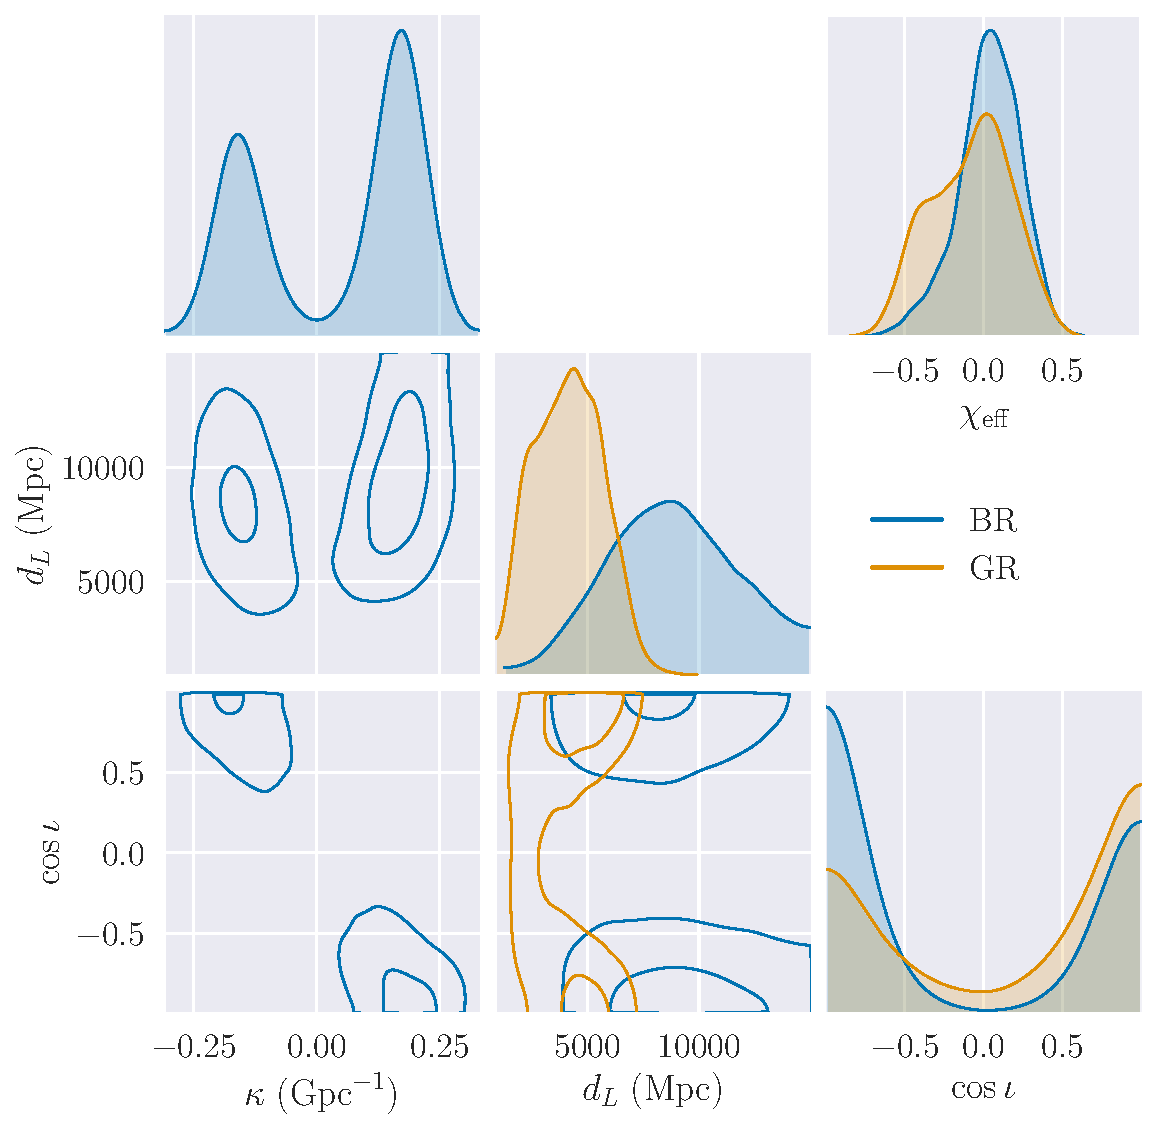
\includegraphics[width=\columnwidth]{figures/corner_GW190521.pdf}
    \caption{
        The posterior of $\kappa$, luminosity distance $d_L$ and $\cos{\iota}$ for GW190521.
        Colors in the plot are the PE result with GR done by LVK without cosmological reweighing \citep{GWTC-2.1, GWTC-3} and the PE result done by us with the frequency-dependent birefringence.
        2D contour plot shows $39.35\%$ and $90\%$ confidence level.
        This plot shows that frequency-dependent birefringence cannot break the degeneracy between $\kappa$ and $\iota$.
    }
    \label{fig:corner_GW190521}
\end{figure}

% Case: GW200129 (glitch in Virgo data)
\subsection{Exclusion of GW200129}
\label{sec:GW200129}
The reason for the exclusion is that past research suggests a potential glitch in GW200129 Virgo data. \citep{GW200129_glitch}
We perform three sets of PE to check if the glitch would affect the population posterior of $\kappa$.
We pick only two out of three detector data in each set to perform PE. (i.e. LIGO-Hanford and LIGO-Livingston for the first set, LIGO-Hanford and Virgo for the second set, and LIGO-Livingston and Virgo for the third set.)
The two sets of PE results with Virgo data return a $\kappa$ posterior that strongly suggests a negative $\kappa$.
Further investigation is needed to understand the glitch.
Thus, we did not include this event in our collective analysis.
% show results included and excluded

% Case: GW190720 (failed PE)
\subsection{Exclusion of GW190720}
\label{sec:GW190720}
For GW190720, we could not perform PE with Bilby successfully.
In LVK PE papers \citep{GWTC-2.1, GWTC-3}, the PE of some events was performed with LALInference \citep{lalsuite} instead of Bilby.
GW190720 was one of them.
We successfully migrated the LALInference configuration to Bilby for most of these events and recovered similar PE results, except for GW190720.
Bilby could not evaluate the likelihood function on Virgo data.
As a result, we excluded this event from our analysis.

\section{Discussion}
\label{sec:Discussion}

% Comparison with previous studies
\subsection{Comparison with previous studies}
\citet{Okounkova_2022} gave a constraint on GW amplitude birefringence by performing statistical analysis on GWTC-2.
We convert the constraint they gave to the same units as ours to make a comparison.
They were able to constrain $\kappa$ to be $|\kappa| \lesssim 0.74$ at $1 \sigma$.
We obtained a tighter constraint on $\kappa$ with $|\kappa| \lesssim 0.04$ at $1 \sigma$.
Our result is an order of magnitude improvement in constraining $\kappa$.
The main reason is that we have more events from GWTC-3 than GWTC-2.

\citet{Wang_2021} performed PE on GWTC-1 events with a frequency-dependent birefringence model.
They formulated the birefringence effect as corrections to the GW waveform on a linear basis.
We convert their constraint to the same units as ours with the derivation in Appendix~\ref{sec:M_PV_derivation}.
% Discussion on the difference between our work and theirs

% Future work
\subsection{Future work}
% BNS
Future work is to perform PE on binary neutron star mergers, such as GW170817.
The frequency range of the signal is much wider compared to the binary black hole mergers.
Thus, the difference in the effect of birefringence at different frequencies within the range can be more significant.
The PE on binary neutron star mergers can allow us to further constrain the birefringence effect and the beyond-GR theories that predict it.
However, performing PE on binary neutron star mergers requires much more computational resources.
Therefore, we may need to wait for future PE methods and tools to further our work.

% More observations with higher SNR
Another future work is to apply the same method to more GW events and events with a higher signal-to-noise ratio (SNR).
LVK will release more events with higher SNR in the future.
Using data with higher SNR allows us to obtain more precise PE results and constrain the birefringence effect more precisely.
And using data from more events will allow us to calculate a more constrained population posterior of $\kappa$.

\begin{acknowledgments}
M.~I., K.~W.~K.~W.~, and W.~M.~F.~ are funded by the Center for Computational Astrophysics at the Flatiron Institute.
The Flatiron Institute provided the computational resources used in this work.

This research has made use of data or software obtained from the Gravitational Wave Open Science Center (gwosc.org), a service of LIGO Laboratory, the LIGO Scientific Collaboration, the Virgo Collaboration, and KAGRA.
LIGO Laboratory and Advanced LIGO are funded by the United States National Science Foundation (NSF) as well as the Science and Technology Facilities Council (STFC) of the United Kingdom, the Max-Planck-Society (MPS), and the State of Niedersachsen/Germany for support of the construction of Advanced LIGO and construction and operation of the GEO600 detector.
Additional support for Advanced LIGO was provided by the Australian Research Council.
Virgo is funded, through the European Gravitational Observatory (EGO), by the French Centre National de Recherche Scientifique (CNRS), the Italian Istituto Nazionale di Fisica Nucleare (INFN) and the Dutch Nikhef, with contributions by institutions from Belgium, Germany, Greece, Hungary, Ireland, Japan, Monaco, Poland, Portugal, Spain.
KAGRA is supported by Ministry of Education, Culture, Sports, Science and Technology (MEXT), Japan Society for the Promotion of Science (JSPS) in Japan; National Research Foundation (NRF) and Ministry of Science and ICT (MSIT) in Korea; Academia Sinica (AS) and National Science and Technology Council (NSTC) in Taiwan.
\end{acknowledgments}

\appendix

\section{Relation between $\kappa$ and $M_{PV}$}
\label{sec:M_PV_derivation}

\citet{Wang_2021} formulated the birefringence effect as
\begin{equation}
    h_{+/\times}^{PV}(f) = h_{+/\times}^{GR}(f)\mp h_{\times/+}^{GR}(f)(i\delta h-\delta\Psi)\,,
\end{equation}
where $h_{+/\times}^{PV}(f)$ is the modified \ac{GW} waveform in the linear basis, $h_{+/\times}^{GR}(f)$ is the \ac{GW} waveform in the linear basis as \ac{GR} predicts, $\delta h$ is the amplitude modification, and $\delta\Psi$ is the phase modification.
We can rewrite the equation as
\begin{equation}
\begin{split}
    h_{L/R}^{PV}(f)&=h_{L/R}^{GR}(f)(1\mp\delta h\mp i\delta\Psi)\\
    &\approx h_{L/R}^{GR}(f)e^{(\mp\delta h\mp i\delta\Psi)}
\end{split}
\,,
\end{equation}
where $h_{L/R}^{PV}(f)$ is the modified \ac{GW} waveform in the circular basis, $h_{L/R}^{GR}(f)$ is the \ac{GW} waveform in the circular basis as \ac{GR} predicts.
This equation applies to any birefringence model that allows the assumption that the modification to \ac{GR} is small when observed very near the source.
To make a comparison with our work, we can choose $\delta\Psi=0$, which is a case that \citet{Wang_2021} considered.
In their work, they parametrized $\delta h=-A_\nu\pi f$, while
\begin{equation}
    A_\nu=M_{PV}^{-1}(\alpha_\nu(z=0)-\alpha_\nu(z)(1+z))\,,
\end{equation}
where $A_\nu$ is the parity-violating parameter for amplitude birefringence, $M_{PV}$ is the characteristic energy scale, and $\alpha_\nu$ is a arbitrary functions determined by the birefringence model.
They then chose $\alpha_\nu=1$.
Therefore, we can rewrite the equation as
\begin{equation}
    h_{L/R}^{PV}(f)= h_{L/R}^{GR}(f)\exp\left(\mp\frac{\pi zf}{M_{PV}}\right)\,.
\end{equation}
This equation takes the same form as \eqref{eq:waveform_modification}.
We can then find the relation between $M_{PV}$ and $\kappa$ by
\begin{equation}
    \left|\mp\frac{\pi zf}{M_{PV}}\right|=\left|\pm\kappa\frac{d_C}{1\,\mathrm{Gpc}}\frac{f}{100\,\mathrm{Hz}}\right|\,.
\end{equation}
Using $H_0d_C=cz$, where $H_0$ is the Hubble constant and $c$ is the speed of light, we can rewrite the equation as
\begin{equation}
    \kappa=\frac{\pi H_0}{c}\left(1\,\mathrm{Gpc}\right)\left(100\,\mathrm{Hz}\right)M_{PV}^{-1}\,.
\end{equation}

\section{Illustration of birefringence}
\label{sec:time_domain}

\begin{figure}[h]
    \script{birefringence_time_domain.py}
    \includegraphics[width=\columnwidth]{figures/birefringence_time_domain.pdf}
    \caption{The observed time domain signal with and without birefringence.}
    \label{fig:birefringence_time_domain}
\end{figure}

\section{Corner plots of special events}
\label{sec:corner_plots}

\begin{figure}[h]
    \script{corner_GW170818.py}
    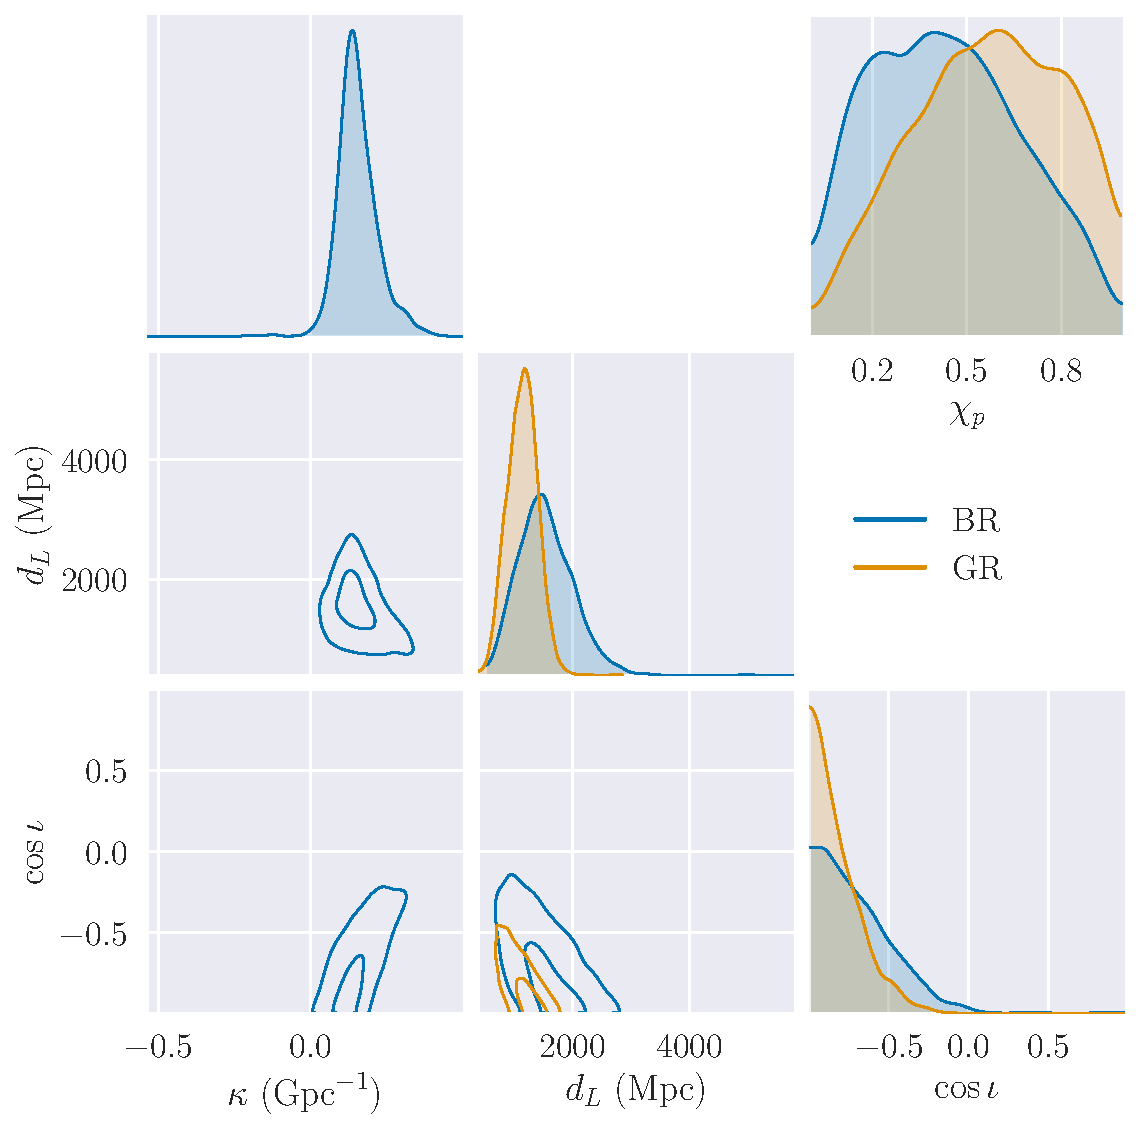
\includegraphics[width=\columnwidth]{figures/corner_GW170818.pdf}
    \caption{Corner plot of GW170818.}
    \label{fig:corner_GW170818}
\end{figure}

\begin{figure}[h]
    \script{corner_GW200129.py}
    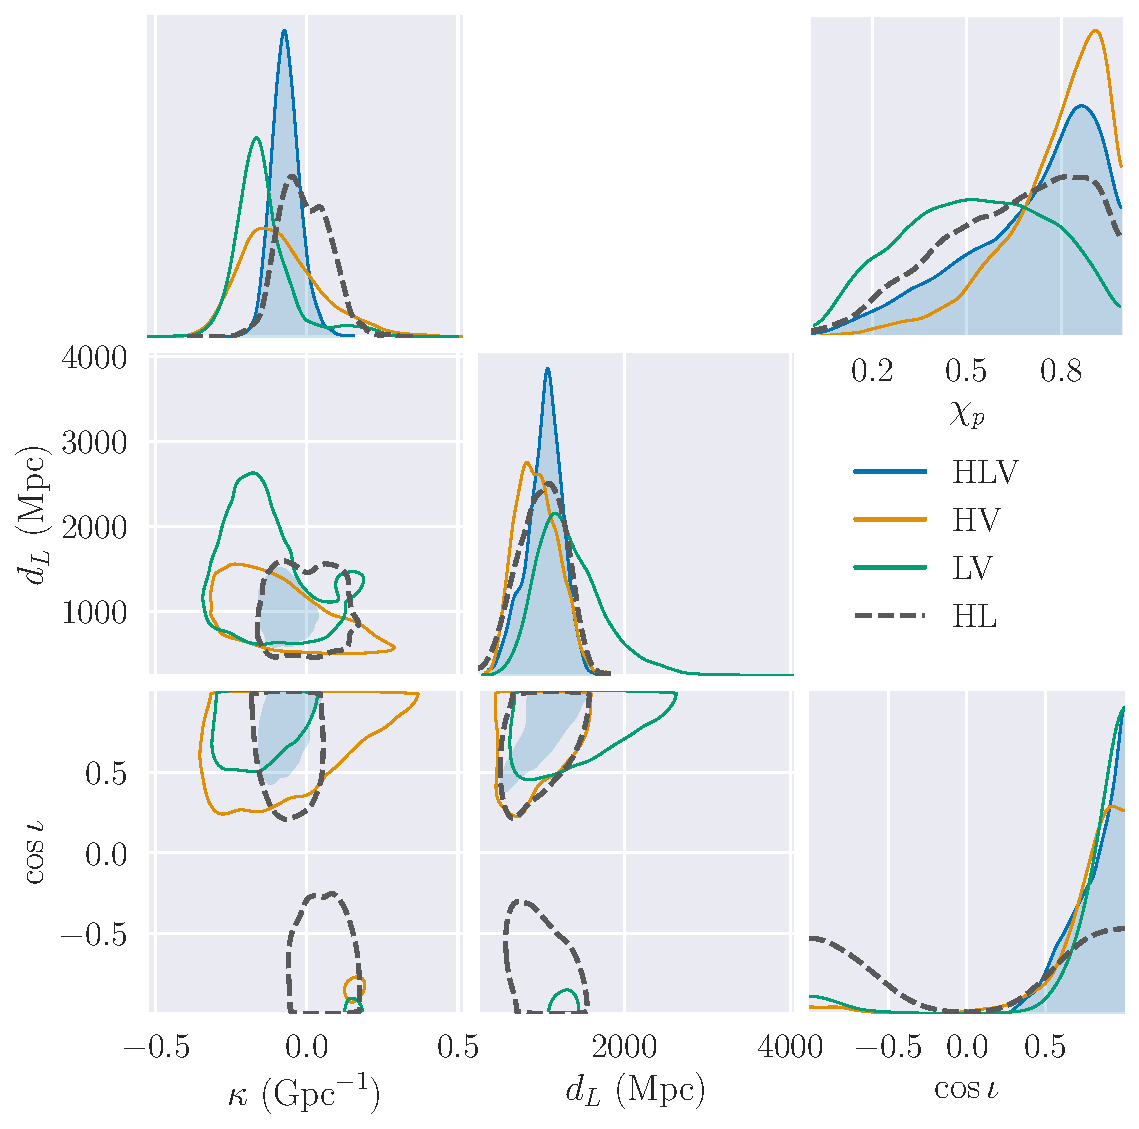
\includegraphics[width=\columnwidth]{figures/corner_GW200129.pdf}
    \caption{Corner plot of GW200129.}
    \label{fig:corner_GW200129}
\end{figure}

\begin{figure}[h]
    \script{corner_GW200224.py}
    \includegraphics[width=\columnwidth]{figures/corner_GW200224.pdf}
    \caption{Corner plot of GW200224.}
    \label{fig:corner_GW200224}
\end{figure}

\bibliography{bib}

\end{document}
